\documentclass{article}
\usepackage{titling}
\usepackage{graphicx}
\usepackage[margin=1in]{geometry}
\usepackage{float}
\usepackage{caption}
\usepackage{subcaption}
\usepackage{tabularx}

\title{CM30225 Parallel Computing
Assessed Coursework Assignment 1}
\preauthor{}
\author{}
\postauthor{}

\begin{document}

\maketitle
\section{Algorithm Design}
My initial design for the algorithm was possibly too naiive; the plan was for all threads to work on the same given matrix, and simply lock the cells that they needed for the calculation whilst in use. 
    \begin{figure}[H]
        \centering
        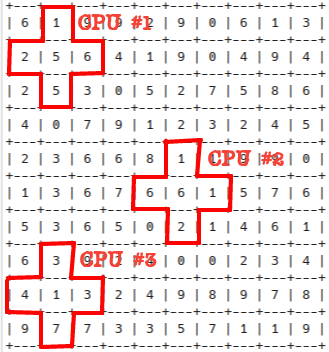
\includegraphics[scale=0.5]{1.png}
        \caption{Naiive Appoach}
        \label{fig1}
    \end{figure}
As can be seen in Figure \ref{fig1}, a thread would lock the current cell, and the cells required to decide the new average, until the calculation was complete. The thread then releases the lock and finds a new cell. Initially, this appears like it would be an acceptable solution, however on reflection, I realized that more time would be spent on overhead - locking cells, checking the status of cells, finding new unlocked cells - than would actually be spent on the main calculation. Thus I decided to find a new algorithm with higher work efficiency, and what follows is the solution I came to.\\
\begin{figure}
    \centering
    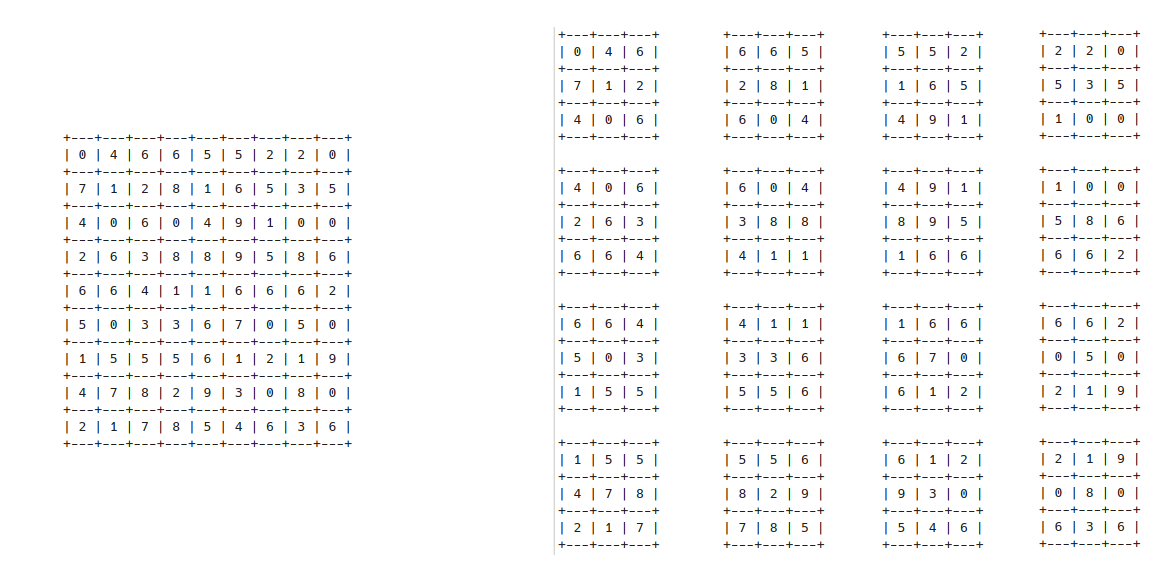
\includegraphics[scale=1.6]{2.png}
    \caption{Scalable Approach}
    \label{fig2}
\end{figure}
\begin{figure}
    \centering
    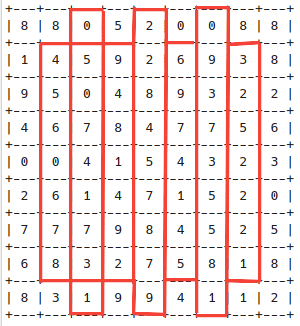
\includegraphics[scale=0.5]{3.png}
    \caption{Boundary computation: First columns, then rows}
    \label{fig3}
\end{figure}
In Figure \ref{fig2}, the matrix is split into \textit{p} sub-matrices, where \textit{p} is the number of processors the program is to run on, and each sub-matrices boundary overlaps its neighbours (In Figure \ref{fig2}, it is assumed there are 16 processors to run on). The process runs as expected, with each thread computing the inner values of its matrix to the desired precision, and leaving the boundaries untouched.
Then sub-matrices will be merged, and their boundaries computed. If the initial matrix is of an odd size (i.e. 9x9), their boundaries will be computed as a $3*n$ array, where $n$ is the size of the $n*n$ square array provided. The first pass will be columns, and then second pass is rows (See Figure \ref{fig3}). For even arrays, one set of sub-matrices will have an extra column/row, so computation will be marginally slower for even arrays.\\
As seen in Figure \ref{fig3}, The arrays passed to each processor will overlap, however since the shared values have already been computed to the desired precision and won't be changed, this shouldn't cause any issues. \\
This is my initial consideration of the algorithm design, pre-development. There is obviously room for improvement; for example, if the number of processors \textit{p} does not evenly fit into the $(n+1)^2$ sub-matrices generated (as in Figure \ref{fig2}), what should be done? Clearly, the division of the matrix into an efficient number of sub-matrices can be improved, however I maintain that this principle of overlapping sub-matrices and then subsequently computing boundaries along columns/rows appears to be a good approach.
\subsubsection{Final Algorithm}
After much painstaking deliberation, what I believe to be the optimal algorithm has been found. It is a halfway compromise between the initial random-find-and-lock algorithm and the overly complicated divide-and-conquer algorithm.\\\newline
\begin{figure}
    \centering
    \begin{subfigure}{.5\textwidth}
      \centering
      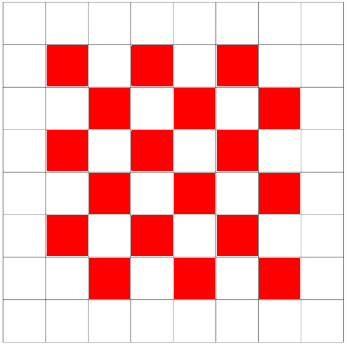
\includegraphics[width=.4\linewidth]{4.png}
      \caption{First Pass}
      \label{fig:sub1}
    \end{subfigure}%
    \begin{subfigure}{.5\textwidth}
      \centering
      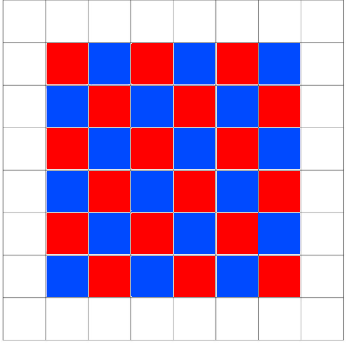
\includegraphics[width=.4\linewidth]{5.png}
      \caption{Second Pass}
      \label{fig:sub2}
    \end{subfigure}
    \caption{Matrix Passes of the Algorithm}
    \label{fig4}
    \end{figure}
As can be seen in figure \ref{fig4}, If the diagonals of the matrix are taken, and the red cells have their values calculated, there is no interference between threads. In the second pass, the opposite diagonals are calculated, and the computation is complete. The intuitive way to perform this calculation is as follows:
\begin{figure}[H]
    \begin{enumerate}
        \item The diagonal cells in Figure \ref{fig:sub1} are identified; this is Pass \#1
        \item The diagonal cells in Figure \ref{fig:sub2} are identified. this is Pass \#2
        \item The number of items in Pass \#1 is divided by the number of threads for the process to run on. This gives us the number of cells each thread must process, $n$.
        \item The same is done for Pass \#2, $m$.
        \item Each thread is randomly assigned $n$ exclusive items from Pass \#1, and $m$ items for Pass \#2.
        \item The threads perform their calculations.
        \item Threads will check if there is any change in the auxillary cells (i.e. the cells required to calculate the average) of the Pass \#2 cells. If there is not, they set a flag.
        \item Once all threads have completed Pass \#1, they are free to move on to Pass \#2.
        \item The computation for Pass \#2 is performed.
        \item The threads check again, but this time for Pass \#1 cells. If the flag was set from step 7, and this check is also successful, the calculation is complete and the thread marks itself as finished. If not, the process repeats from step 6.
    \end{enumerate}
    \caption{Algorithm Flow}
    \label{algo}
\end{figure}
This algorithm at first glance appears to elegantly avoid all race conditions and maximise the work throughput of threads. \newpage
\section{Implementation}
This section is best read as an accompanying document when reading the source code.\\\newline
The interface of the program is as follows:
\begin{figure}[H]
    \begin{verbatim}
    Usage: main [options]
    Options: 
        -P      double; the desired precision to work to.
        -p      int; number of threads to run on. (Note: one thread is a control thread
                only p-1 threads will run the computation).
        -n      int; the dimension of the provided array (must be square).
        -a      space-separated list of integers or doubles; the array to be computed
                integers will be converted to doubles.
        -af     file; the array provided in a file. Each element must have its own line.
        \end{verbatim}
        \caption{Program Interface}
        \label{progint}
\end{figure}
For convenience, a simple Makefile was used to compile the program with the required libraries and subsequently run the program with some set of parameters. Behaviour for incorrect parameters, or an insufficient number of parameters, is not defined (as it did not appear to be the purpose of the coursework).
Some notes on the code: 
\subsection{main function: compute()}
compute() is the main function of the program. Its interface is as follows:
\begin{center}
    \begin{verbatim}
double **compute(int p, double P, int n, double **a)
    \end{verbatim}
\end{center}
which corresponds to the parameters defined in Figure \ref{progint}. Without going into excessive detail, this function:
\begin{enumerate}
    \item  Identifies the cells in Pass \#1 and \#2 from Figure \ref{fig4}
    \item   Divides the work between the threads
    \item Creates threads
    \item Checks if threads are done; upon completion it returns array $a$.
\end{enumerate}
The function that each thread is given to execute is multi-parameter, so a struct \textbf{ARGT} is created with the necessary values, which is then passed through \textbf{pthread\_create()}.
\subsection{thread function: compute0()}
compute0() is the function that the slave threads (in contrast to the control thread which runs \textbf{compute()}) run. compute1() is the sequential analogue of this function that will be used to test correctness and to evaluate efficiency later on. 
compute0() implements 3 thread barriers, for which each of the slave threads must reach before they can continue to execute. These are; $check$, $passa$, and $passb$. The purpose of $passa$ and $passb$ should be fairly self explanatory from the description in Figure \ref{algo}, and the $check$ barrier is used to make sure all passes are finished before the check is done. compute0 is an infinite loop, where threads only have the ability to set a flag signalling their status and not cancel themselves. This was because of a technicality where, if a given thread cancelled itself before others, the barrier could not be passed and the threads would hang. As a result of this, the control thread now performs all thread management.
\subsection{Auxiliary Functions and Structures}{
\subsubsection{structs}
 \begin{table}[H]
    \renewcommand*{\arraystretch}{1.2}
    \begin{tabularx}{\textwidth}{|l|X|}
        \hline 
        \textbf{CELL} & The cell information for each thread of which cells to compute - a linked list whose values contain the (x,y) coordinates, the current value, the previous value, and the previous 4 values of its neighbours.\\ \hline
        \textbf{TSTAT} & Holds the status of each thread; whether is has finished its computation, and the number of passes it made.\\\hline
        \textbf{ARGT}  & The argument object passed to compute() because of the one-argument restriction on \textbf{pthread\_create()}. Contains $P$, $a$ (the same as the values from the interface in Figure \ref{progint}), and two \textbf{CELL}s, for Pass \#1 and Pass \#2 respectively.\\\hline
    \end{tabularx}
 \end{table}
 \subsubsection{functions}
 \begin{table}[H]
    \renewcommand*{\arraystretch}{1.2}
    \begin{tabularx}{\textwidth}{|l|X|}
        \hline 
        \textbf{new\_tstat() update\_tstat() find\_tstat()} & functions to create a \textbf{TSTAT}, for a thread to mark itself complete and to find a tstat by thread id respectively. \\ \hline
        \textbf{new\_workt()} & Returns a group of work for a thread. Takes the linked list of \textbf{CELL}s $a$, and returns the first $n$ elements of the list, where n is the work for a given thread. \\ \hline
        \textbf{check\_done()} & Checks if a thread is done. Takes the absolute value of the difference between the current and previous values of the auxillary cells for each cell in a threads workload, and checks if their sum is less than or equal to $P*4$, since when averaged out they would not change the value more than the desired precision. \\ \hline
    \end{tabularx}
\end{table}
There are a few more functions in the program, however they are all self explanatory and are not worth mentioning; the above should be sufficient for understanding the function of the program.
\section{Analysis}
\subsection{Scalability Investigation}
\subsubsection{Efficency}
Running on 43 threads with an matrix of dimension $n=1000$, the program completes in 57 seconds flat. The same size matrix completes sequentially in 
\subsection{Correctness Testing}
\end{document}
